\section{Deriving the Dirac's equation}
As we saw in the previous chapter, the Klein-Gordon equation \eqref{KleinGordonEq} is unable to describe a relativistic theory of quantum mechanics that, as for the classical formulation from Schrödinger, can result in a probabilistic interpretation of the wave function. Furthermore, we will see that the new theory that we are going to describe, predicts precisely all of those aspects that are shown by experiments but that in classical quantum mechanics (as well for the Klein-Gordon theory) needs to be "artificially" added.\\

Dirac understood that absence of a definite positive probability density, in the Klein-Gordon equations, was caused by the non-linearity of the differential equation, with respect to time. Since quantizing the energy momentum relation of the form $E=\sqrt{c\vec p^2+m^2c^4}$ had its own problems, as we already discussed in Section \ref{sec:FromClassicalToRelativisticQM}, Dirac tried a different approach: he assumed that was possible to obtain a linear relation between momentum and energy using a set of four hermitian\footnote{These must be hermitian since the whole expression has to be real: in this way E is hermitian too and thus its components, since it is a multiple of the identity matrix $4\times4$, are real.} matrix:
\begin{equation}\label{DiracAssumption}
    E=c\vec\alpha\cdot\vec p+\beta mc^2,\qquad \alpha_1,\alpha_2,\alpha_3,\beta\in M_{4\times4}(\mathbb{C}).
\end{equation}
Given this assumption, we need to have it satisfy the energy momentum relation:
\begin{align*}
    E^2&=(c\alpha^i p^i+\beta mc^2)(c\alpha^j p^j+\beta mc^2)\\&=cp^ip^j\alpha^i\alpha^j+\beta^2m^2c^4+mc^3p^i\bigl(\alpha^i\beta+\beta\alpha^i\bigr)\\&=c^2\vec p^2+m^2c^4.
\end{align*}
In order to have this last equality satisfied we need:
\begin{itemize}
    \item $\beta^2=1\quad \Rightarrow\quad \{\beta,\beta\}=2$;
    \item $\alpha^i\beta+\beta\alpha^i=0\quad \Rightarrow\quad \{\beta,\alpha^i\}=0,\ i=\{1,2,3\}$;
    \item since $p^ip^j$ is symmetric, the symmetric part\footnote{Any symmetric tensor contracted with an antisymmetric one always vanishes.} of $\alpha^i\alpha^j$ should result in a Kronecker's delta
    \begin{equation*}
        \frac{\alpha^i\alpha^j+\alpha^j\alpha^i}{2}=\delta^{ij}\quad \Rightarrow\quad \{\alpha^i\alpha^j\}=2\delta^{ij},\ i,j=\{1,2,3\}.
    \end{equation*}
\end{itemize}
The notation $\{A,B\}$ is the anticommutator: $AB+BA$.\\
This structure defines a \emph{Clifford algebra} and can be used to derive the explicit form of these matrices (we use a shorthand notation for $4\times4$ matrices):
\begin{align}\label{DiracMatrixAB}
    \beta=\begin{pmatrix}
        \mathds{1}&&0\\
        0&& -\mathds{1}
    \end{pmatrix},\qquad
    \alpha^i=\begin{pmatrix}
        0 && \sigma^i\\
        \sigma^i&& 0
    \end{pmatrix},
\end{align} 
where $\sigma^i$ are the $2\times2$ Pauli matrices
\begin{equation}\label{PauliMatrix}
    \sigma^1=\begin{pmatrix}
        0&&1\\
        1&&0
    \end{pmatrix},\quad
    \sigma^2=\begin{pmatrix}
        0&&-i\\
        i&&0
    \end{pmatrix},\quad
    \sigma^3=\begin{pmatrix}
        1&&0\\
        0&&-1
    \end{pmatrix}.
\end{equation}
We now need to quantize equation \eqref{DiracAssumption}. In order to do so we promote observable to operators acting on wave functions (as in Section\ref{sec:FromClassicalToRelativisticQM}):
\begin{equation*}
    E\rightsquigarrow i\hslash\partial_t,\qquad\vec p\rightsquigarrow -i\hslash\vec\nabla.
\end{equation*} 
Before plugging this operator inside the equation \eqref{DiracAssumption} we have to stress the fact that those operators are multiplied to some $4\times4$ matrices (Eq. \eqref{DiracMatrixAB}) and thus we cannot expect to have a scalar wave function. It is natural to use a vector of $4$ wave functions, called \textbf{spinor}\index{spinor}. The resulting equation reads:
\begin{equation*}
    i\hslash\partial_t\psi=(-ic\hslash\alpha^i\partial_i+\beta mc^2)\psi.
\end{equation*}
We now want to express this equation in a covariant form: to do so we define:
\begin{equation}\label{DiracMatrixG}
    \gamma^0=-i\beta,\qquad \gamma^j=-i\beta\alpha^j,\qquad j=\{1,2,3\}.
\end{equation}
In this way, multiplying ,at the left, both sides of the above equation by $\frac{\beta}{c\hslash}$, remembering that $\beta^2\mathds{1}$ and plugging the matrices \refeq{DiracMatrixG}, we get:
\begin{align*}
    &\frac{i\beta}{c}\partial_t\psi=\bigg(-i\beta\alpha^i\partial_i+\frac{mc}{\hslash}\bigg)\psi\\&\Rightarrow\bigg(\gamma^0\partial_0+\gamma^i\partial_i\frac{mc}{\hslash}\bigg)\psi=0
    \\&\Rightarrow\bigg(\gamma^\mu\partial_\mu+\frac{mc}{\hslash}\bigg)\psi=0.
\end{align*}
Lastly we use the natural units with the Feynman's slash convention $\not\partial= \gamma^\mu\partial_\mu$, it reads:
\begin{equation}
    \label{DiracEquation}(\not\partial+m)\psi=0.
\end{equation}
We remind that $\psi(x^\mu)$ is a vector of four wave functions:
\begin{equation*}
    \psi(x^\mu)=\begin{pmatrix}
    \psi_1(x^\mu)\\\psi_2(x^\mu)\\\psi_3(x^\mu)\\\psi_4(x^\mu)
    \end{pmatrix}, \qquad \psi_i:\mathbb{R}^4\rightarrow\mathbb{C}. 
\end{equation*}

Let's now check if this equation has some kind of probability current and density. First we can multiply, to the left, the equation \eqref{DiracEquation} by $\psi^\dagger$, then we subtract the conjugate transpose of the same equation, multiplied by $\psi$ to the left:
\begin{align*}
    0&=\psi^\dagger\big[\gamma^\mu\partial_\mu+m\big]\psi-\big[\big(\gamma^\nu\partial_\nu+m\big)\psi\big]^\dagger\psi\\
    &=\psi^\dagger\big[\gamma^\mu\partial_\mu+m\big]\psi-\big[\partial_\nu\psi^\dagger\gamma^{\dagger\nu}+\psi^\dagger m\big]\psi\\
    &=\psi^\dagger\gamma^\mu\partial_\mu\psi+\partial_\mu\psi^\dagger\gamma^\mu\psi=\partial_\mu\big(\psi^\dagger\gamma^\mu\psi\big).
\end{align*}  
We have obtained a conserved quantity in a form of \emph{continuity equation}, as it happens with the Schrödinger equation, thus we can conclude that Dirac's approach restore the probability interpretation of quantum mechanics. It is more convenient to multiply the continuity equation by $i\beta$, in this way $\big(i\beta\gamma^0=\beta^2=\mathds{1}\big)$ the probability density reads $\psi^\dagger\psi$ as in classical quantum mechanics.
\subsection{Some proprieties of the $\gamma$ matrices}
We will now discuss the main proprieties of the matrix formalism \refeq{DiracMatrixG} introduced by Dirac.\\
First of all we should notice that, since $\beta $ and $\alpha^i$ form a Clifford algebra, the corresponding $\gamma^0=-i\beta,\ \gamma^j=-i\beta\alpha^j$ form the same structure:
\begin{equation*}
    \{\gamma^\mu,\gamma^\nu\}=2\eta^{\mu\nu}.
\end{equation*}
Furthermore, from the hermiticity of $\beta $ and $\alpha^i$ and the anticommutation relation $\beta\alpha^i=-\alpha^i\beta$, it is easy to see that $\gamma^0$ is antihermitian and $\gamma^i$ are hermitian:
\begin{equation*}
    \big(\gamma^0\big)^\dagger= \big(-i\beta\big)^\dagger=i\beta=-\gamma^0,\quad\big(\gamma^j\big)^\dagger= \big(-i\beta\alpha^j\big)^\dagger=i\alpha^j\beta=-i\beta\alpha^j=\gamma^j.
\end{equation*}
These relations can be summarized in the compact form
\begin{equation*}
    \big(\gamma^\mu\big)^\dagger=\gamma^0\gamma^\mu\gamma^0\quad\text{or}\quad\big(\gamma^\mu\big)^\dagger=-\beta\gamma^\mu\beta.
\end{equation*}
The second proprieties of these matrices is that are traceless, for example, using that $\big(\gamma^2\big)^2=\mathds{1}$, the anticommutation and the cyclic propriety of the trace:
\begin{equation*}
    Tr\ \gamma^1=Tr\ \gamma^1\big(\gamma^2\big)^2=-Tr\ \gamma^2\gamma^1\gamma^2=-Tr\ \gamma^1\big(\gamma^2\big)=-Tr\ \gamma^1\quad\Rightarrow\quad Tr\ \gamma^1=0.
\end{equation*}
Lastly we should introduce the \textbf{chirality matrix} $\gamma^5$, defined by
\begin{equation}\label{ChiralityMatrix}
    \gamma^5=-i\gamma^0\gamma^1\gamma^2\gamma^3,
\end{equation}
which has the following proprieties:
\begin{equation}
    \{\gamma^5,\gamma^\mu\}=0,\quad \big(\gamma^5\big)^2=\mathds{1},\quad \big(\gamma^5\big)^\dagger=\gamma^5,\quad Tr\ \gamma^5=0.
\end{equation} 
This matrix is needed to define the \textbf{chiral projectors}
\begin{equation}
    \label{ChiralProjectors} P_L=\frac{\mathds{1}-\gamma^5}{2},\quad P_R=\frac{\mathds{1}+\gamma^5}{2}
\end{equation}
that allows the Dirac spinor to be divided into its right-handed and left-handed components, called \textbf{Weyl spinors}.
\section{Plane wave solution of Dirac's equation}
We will now study the problem of finding the free particle solutions of the Dirac's equation.\\In order to do so we will suppose that a solution will be in the form:
\begin{equation*}
    \psi(x^\mu)=\omega(P^\mu)e^{iP_\mu x^\mu},
\end{equation*}
where $P^\mu$ is an arbitrary 4-vector and $\omega$ is the \textbf{polarization spinor}.\\
Plugging this ansatz in the Eq. \eqref{DiracEquation} we get the following condition:
\begin{equation*}
    0=\big(\gamma^\mu\partial_\mu+m\big)\omega(P^\mu)e^{iP_\nu x^\nu}=\big(i\gamma^\mu P_\mu+m\big)\omega(P^\mu)e^{iP_\nu x^\nu}.
\end{equation*} 
By multiplication by $\big(-i\gamma^\nu P_\nu+m\big)$ and observing that
\begin{equation*}
    P^\mu P^\nu \gamma^\mu \gamma^\nu=P^\mu P^\nu\frac{\gamma^\mu\gamma^\nu+\gamma^\nu\gamma^\mu}{2}=P^\mu P^\nu\eta^{\mu\nu}=P^\mu P_\mu,
\end{equation*}
we than get the condition needed to have our ansatz to satisfy the Dirac's equation:
\begin{equation*}
    \big(P^\mu P_\mu+m^2\big)\omega(P^\mu)=0,
\end{equation*}
where we can recognize the mass-shell condition and thus that $P^\mu$ has to be the 4-momentum.\\
Let's now consider a rest particle, therefore its 4-momentum will be $P^\mu=(E,0,0,0)$. In this case the first condition we obtained reads:
\begin{equation*}
    0=(i\gamma^0P_0+m)\omega=(-iE\gamma^0+m)\omega=(E\beta+m)\omega.
\end{equation*}
In matrix form:
\begin{equation*}
    \begin{pmatrix}
        E&&0&&0&&0\\
        0&&E&&0&&0\\
        0&&0&& E&&0\\
        0&&0&&0&&E
    \end{pmatrix}
    \begin{pmatrix}
        \omega_1\\\omega_2\\\omega_3\\\omega_4
    \end{pmatrix}
    =\begin{pmatrix}
        m&&0&&0&&0\\
        0&&m&&0&&0\\
        0&&0&& -m&&0\\
        0&&0&&0&&-m
    \end{pmatrix}
    \begin{pmatrix}
        \omega_1\\\omega_2\\\omega_3\\\omega_4
    \end{pmatrix},
\end{equation*}
it is clear that even Dirac's equation allows some negative energy states ($E=-m$) which are characterized by different polarization spinor with respect to those with positive energy
\begin{equation*}
    \omega=\begin{pmatrix}
        1\\0\\0\\0
    \end{pmatrix},
    \begin{pmatrix}
        0\\1\\0\\0
    \end{pmatrix}\rightarrow \text{Positive energy},\qquad
    \omega=\begin{pmatrix}
        0\\0\\1\\0
    \end{pmatrix},
    \begin{pmatrix}
        0\\0\\0\\1
    \end{pmatrix}\rightarrow \text{Negative energy}.
\end{equation*}
Solutions for a particle at rest will then read:
\begin{equation*}
    \psi(x^\mu)=\omega(P^\mu)e^{-imt},
\end{equation*}
we will obtain solutions describing moving particles performing boots on these solutions.
\section{Non-relativistic limit of the Dirac's equation}
In order to test the validity of this theory we can study the limit for which this should reduce to the classical one and verify if those two are consistent. Furthermore, this approach will give us easier equation that can be used as correction to the classical theory.\\

First of all we have to take into accounts that classical quantum mechanics make use of 2-d spinors, and for this reason we divide the Dirac's spinors in two components (we have again introduced non-natural units because we will need to study the limit $c\rightarrow\infty$):
\begin{equation*}
    \psi=\begin{pmatrix}
        \psi_1\\\psi_3\\\psi_3\\\psi_4
    \end{pmatrix}e^{-\frac{i}{\hslash}mc^2t}
    =\begin{pmatrix}
        \varphi\\\chi
    \end{pmatrix}e^{-\frac{i}{\hslash}mc^2t},\quad \text{such that}\quad
    \varphi=\begin{pmatrix}
        \psi_1\\\psi_2
    \end{pmatrix},\ 
    \chi=\begin{pmatrix}
        \psi_3\\\psi_4
    \end{pmatrix}.
\end{equation*}
Using this notation we get that the Dirac's equation \eqref{DiracEquation} reads ($\vec p$ will be used as a shorthand for the momentum operator):
\begin{align*}
    &i\hslash\partial_t\begin{pmatrix}
        \varphi\\\chi
    \end{pmatrix}e^{-\frac{i}{\hslash}mc^2t}=(c\vec\alpha\cdot\vec p+\beta mc^2)\begin{pmatrix}
        \varphi\\\chi
    \end{pmatrix}e^{-\frac{i}{\hslash}mc^2t}\\
    &i\hslash\bigg[\begin{pmatrix}
        \dot\varphi\\\dot\chi
    \end{pmatrix}+mc^2
        \begin{pmatrix}
            \varphi\\\chi
        \end{pmatrix}\bigg]e^{-\frac{i}{\hslash}mc^2t}
        =\bigg[c
        \begin{pmatrix}
            0&&\vec p\cdot\vec\sigma\\
            \vec p\cdot\vec\sigma&&0
        \end{pmatrix}
        \begin{pmatrix}
            \varphi\\\chi
        \end{pmatrix}+mc^2
        \begin{pmatrix}
            \varphi&&0\\0&&-\chi
        \end{pmatrix}
        \bigg]e^{-\frac{i}{\hslash}mc^2t}
        \\&\Rightarrow\begin{cases}
            i\hslash\dot\varphi+mc^2\varphi=c\vec\sigma\cdot\vec p\chi+mc^2\varphi\\
            i\hslash\dot\chi+mc^2\chi=c\vec\sigma\cdot\vec p\varphi-mc^2\chi
        \end{cases}.
\end{align*}
The first equation we have obtained contains some terms that cancel out, while the second one is the one that should be treated in order to get the non-relativistic limit:
\begin{equation*}
    \begin{cases}
        i\hslash\dot\varphi=c\vec\sigma\cdot\vec p\chi\\
        i\hslash\dot\chi+2mc^2\chi=c\vec\sigma\cdot\vec p\varphi
    \end{cases},
\end{equation*}
this limit can be achieved by considering $c\rightarrow\infty$ and by neglecting smaller term, such as the term $i\hslash\dot\chi$ which will have a negligible contribution with respect to the mass term, which contains $c^2$
\begin{equation*}
    \begin{cases}
        i\hslash\dot\varphi=c\vec\sigma\cdot\vec p\chi\\
        2mc^2\chi=c\vec\sigma\cdot\vec p\varphi
    \end{cases}.
\end{equation*}
Operating the right algebraic substitution we finally get the non-relativistic equation of motion, know as the \textbf{free Pauli's equation}:
\begin{equation*}
    i\hslash\dot\varphi =\frac{(\vec\sigma\cdot\vec p)^2}{2m}\varphi,
\end{equation*}
which, remembering that $\sigma_i\sigma_j=\mathds{1}\delta_{ij}+i\epsilon_{ijk}\sigma_k$, is just the classical Schrödinger's equation.\\

We will now see that, considering electromagnetism, we can recover, in this classical limit, a theory which predicts the spin approach of Pauli, which is normally imposed in classical quantum mechanics.\\To do so we will need to use the generalized momentum:
\begin{equation*}
    \pi_\mu=P_\mu-\frac{e}{c}A_\mu,\quad P^\mu\rightarrow\pi^mu,
\end{equation*}
this technique takes the name of \emph{minimal substitution}. In this way, the Dirac's equation reads:
\begin{equation*}
    i\hslash\partial_t\begin{pmatrix}
        \varphi\\\chi
    \end{pmatrix}e^{-\frac{i}{\hslash}mc^2t}=(c\vec\alpha\cdot\vec\pi+\beta mc^2+e\phi)\begin{pmatrix}
        \varphi\\\chi
    \end{pmatrix}e^{-\frac{i}{\hslash}mc^2t},
\end{equation*}
where $\vec\pi=-i\hslash\vec\nabla-\frac{e}{c}\vec A$.\\
Following the same approach as before we now get:
\begin{equation*}
    \begin{cases}
        i\hslash\dot\varphi=c\vec\sigma\cdot\vec\pi\chi+e\phi\varphi\\
        i\hslash\dot\chi+2mc^2\chi=c\vec\sigma\cdot\vec p\varphi+e\phi\chi
    \end{cases},
\end{equation*}
where the terms $i\hslash\dot\chi$ and $e\phi\chi$ are negligible in the non-relativistic limit $c\rightarrow \infty$. In this limit this reads:
\begin{equation*}
    \begin{cases}
        i\hslash\dot\varphi=c\vec\sigma\cdot\vec\pi\chi+e\phi\varphi\\
        2mc^2\chi=c\vec\sigma\cdot\vec p\varphi
    \end{cases}\qquad\Rightarrow\qquad i\hslash\dot\varphi=\frac{(\vec\sigma\cdot\vec\pi)^2}{2m}+e\phi\varphi.
\end{equation*}
Now we cannot recover the Schrödinger's equation we could get by just classically adding the electromagnetic potentials terms. Expanding the squared term we get:
\begin{equation*}
    \sigma^i\sigma^k\pi^i\pi^k=(\mathds{1}\delta^{ij}+i\epsilon^{ijk}\sigma^{k})\pi^i\pi^k.
\end{equation*}
Since $\epsilon^{ijk}$ is antisymmetric, only the antisymmetric part of $\pi^i\pi^j$ will not vanish, thus:
\begin{equation*}
    \sigma^i\sigma^k\pi^i\pi^k=\pi^i\pi^i+i\epsilon^{ijk}\sigma^{k}\frac{\pi^i\pi^j-\pi^j\pi^i}{2}=\pi^i\pi^i+\frac{i}{2}\epsilon^{ijk}\sigma^{k}[\pi^i,\pi^j].
\end{equation*}
The commutator can be evaluated observing that $[\partial^i,\partial^j]=[A^i,A^j]=0$ and that
\begin{equation*}
    [p^i,A^j]\varphi=-i\hslash\partial^i(\varphi A^j)+i\hslash A^j\partial^i\varphi=-i\hslash A^j\partial^i\varphi -i\hslash\varphi \partial^iA^j+i\hslash A^j\partial^i\varphi=-i\hslash\varphi \partial^iA^j,
\end{equation*}
thus giving:
\begin{equation*}
    [\pi^i,\pi^j]=-\frac{e}{c}\big([p^i,A^j]+[A^i,p^j]\big)=-\frac{e}{c}\big([p^i,A^j]-[p^j,A^i]\big)=-\frac{e}{c}\big(\partial^iA^j-\partial^jA^i\big).
\end{equation*}
The equation we've got in the non-relativistic limit, using the cyclic proprieties of $\epsilon_{ijk}$, now reads:
\begin{equation*}
    i\hslash\dot\varphi=\frac{1}{2m}\bigg\{\vec\pi^2-\frac{\hslash e}{c}\epsilon^{ijk}\partial^iA^j\sigma^k\bigg\}\varphi+e\phi\varphi,
\end{equation*}
which recalling $\epsilon^{ijk}\partial^iA^j=\vec\nabla\times\vec A=\vec B$ becomes
\begin{equation*}
    i\hslash\dot\varphi=\frac{1}{2m}\bigg\{\vec\pi^2-\frac{\hslash e}{c}B^k\sigma^k\bigg\}\varphi+e\phi\varphi.
\end{equation*}
We can now compute $\vec\pi^2$ which, remembering that $\vec L=\vec r\times\vec p$ and that for constant magnetic fields $\vec A=\frac{1}{2}\vec B\times\vec r$, becomes:
\begin{align*}
    \vec\pi^2&=\vec p^2+\frac{e^2}{c^2}\vec A^2-\frac{e}{c}(\vec A\cdot\vec p+\vec p\cdot\vec A)=\vec p^2+\frac{e^2}{c^2}\vec A^2-\frac{e}{2c}(\vec B\times\vec r\cdot\vec p+\vec p\cdot\vec B\times\vec r)\\&=\vec p^2+\frac{e^2}{c^2}\vec A^2-\frac{e}{c}\vec r\times\vec p\cdot\vec B=\vec p^2+\frac{e^2}{c^2}\vec A^2-\frac{e}{c}\vec L\cdot\vec B.
\end{align*}
The full equation reads:
\begin{equation*}
    i\hslash\dot\varphi=\frac{1}{2m}\bigg\{\vec p^2\frac{e^2}{c^2}\vec A^2-\frac{e}{c}\vec L\cdot\vec B-\frac{\hslash e}{c}\vec B\cdot\vec \sigma\bigg\}\varphi+e\phi\varphi,
\end{equation*}
which lastly, defining $\vec S=\frac{\hslash}{2}\vec\sigma$, gives the Pauli's equation with electromagnetic interactions
\begin{equation*}
    i\hslash\dot\varphi=\frac{1}{2m}\bigg\{\vec p^2+\frac{e^2}{c^2}\vec A^2-\frac{e}{c}\big(\vec L\cdot\vec B-2\vec B\cdot\vec S\big)\bigg\}\varphi+e\phi\varphi,
\end{equation*}
In this way we have show that the spin interactions that are imposed in classical quantum mechanics, arise naturally in the Dirac's formalism, even predicting the gyromagnetic factor of $2$ that is measured.

\subsection{The spin operator}
We now generalize the spin operator definition, that we have just given and that is valid in the classical regime, to the Dirac's formalism:
\begin{equation*}
    \vec S=\frac{\hslash}{2}\begin{pmatrix}
        \vec\sigma&&0\\0&&\vec\sigma
    \end{pmatrix}=\frac{\hslash}{2}\Sigma,\qquad\Sigma^i=-\frac{i}{2}\epsilon^{ijk}\alpha^j\alpha^k.
\end{equation*}
Neither this operator, neither the angular momentum operator $L^i=\epsilon^{ijk}x^jp^k$, commute with the hamiltonian of the system (which is given by the Dirac's equation \eqref{DiracEquation}), only their combination $\vec J=\vec S+\vec L$ commutes with the hamiltonian. Using natural units:
\begin{align*}
    \mathcal{H} &=\alpha^l p_l+\beta m,\\
    [\mathcal{H},L^i]&=[\alpha^l p_l,\epsilon^{ijk}x^jp^k]+ [\beta m,\epsilon^{ijk}x^jp^k]\\&=\alpha^l[ p_l,x^j]\epsilon^{ijk}p^k=-i\alpha^l\delta_l^j\epsilon^{ijk}p^k=-i\epsilon^{ijk}\alpha^jp^k,\\
    [\mathcal{H},S^i]&=-\frac{i}{4}[\alpha^l p_l,\epsilon^{ijk}\alpha^j\alpha^k]- \frac{i}{4}[\beta m,\epsilon^{ijk}\alpha^j\alpha^k],\\
    [\beta ,\alpha^j\alpha^k]&=\alpha^j[\beta ,\alpha^k]+[\beta,\alpha^j]\alpha^k\\&=\{\beta ,\alpha^j\}\alpha^k-\alpha^j\{\beta ,\alpha^k\}=0,\\
    [\alpha^l ,\alpha^j\alpha^k]&=\{\alpha^l ,\alpha^j\}\alpha^k-\alpha^j\{\alpha^l, \alpha^k\}\\&=2\delta^{lj}\alpha^k-2\delta^{lk}\alpha^j\\
    [\mathcal{H},S^i]&=-\frac{i}{4}\epsilon^{ijk}(2\delta^{lj}\alpha^k-2\delta^{lk}\alpha^j)p^l=\frac{i}{4}\epsilon^{ijk}(2\delta^{lk}\alpha^j+2\delta^{lk}\alpha^j)p^l\\&=i\epsilon^{ijk}\alpha^jp^k\\
    &\Rightarrow\qquad[\mathcal{H},J^i]=[\mathcal{H},L^i+S^i]=0.
\end{align*}
This shows that degeneracy of energy states can be removed by studying the spectrum of the total angular momentum. This is crucial since, when  studying atomic spectra, only the introduction of spin (that the Klein-Gordon equation doesn't consider) can reproduce the right number of emission/absorption lines.
\section{Relativistic invariance of the Dirac's equation}
In this section we will study the invariance of the Dirac's equation, this will naturally lead us to the internal transformation of the wave function under a Boost, therefore giving us the solution of a particle in motion.\\

First of all, we should remind all the well known transformations of the object we are already familial with:
\begin{equation*}
    x'^\mu=\Lambda^\mu\ _\nu x^\nu,\qquad\partial_\mu^i=\Lambda_\mu\ ^\nu\partial_\nu.
\end{equation*}
We want to find a linear transformation that maps the spinor $\psi$ to the one that satisfy the Dirac's equation in the new reference frame, we will call this transformation $S(\Lambda)\in M_{4\times4}\mathbb{C} $:
\begin{equation*}
    \big(\gamma^\mu\partial'_\mu+m\big)\psi'=\big(\gamma^\mu\Lambda_\mu\ ^\nu\partial_\nu+m\big)S(\Lambda)\psi=0.
\end{equation*}
By multiplying to the left by $S^{-1}$ we obtain
\begin{equation*}
   \big(S^{-1}(\Lambda)\gamma^\mu\Lambda_\mu\ ^\nu S(\Lambda)\partial_\nu+m\big)\psi=0,
\end{equation*}
which should be again some sort of Dirac equation in the old frame of reference. In order to be so $S^{-1}(\Lambda)\gamma^\mu\Lambda_\mu\ ^\nu S(\Lambda)$ should be equal to the Dirac's gammas, giving
\begin{equation*}
    S^{-1}(\Lambda)\gamma^\mu S(\Lambda)=\Lambda^\mu\ _\nu\gamma^\nu,
\end{equation*}
that will be used to derive the explicit form of $S$. \\

We will study what happens under an infinitesimal transformation of the Lorentz Group:
\begin{equation*}
    \Lambda^\mu\ _\nu=\delta^\mu\ _\nu+\omega^\mu\ _\nu\quad\Rightarrow\quad S(\Lambda)=\mathds{1}+\frac{i}{2}\omega_{\mu\nu}\Sigma^{\mu\nu},
\end{equation*}
where $\omega$ are the parameters (small due to the infinitesimal nature) of the transformation (6 in total, such as the angles of rotation or the rapidity of the boost) and $\Sigma$ are some appropriate matrices yet to find. We can show that, from the definition of the Lorentz group (all the transformations that preserve the Minkowski metric), both $\omega_{\mu\nu}$ and $\Sigma^{\mu\nu}$ are antisymmetric. Using the condition obtained by the Dirac's equation:
\begin{align*}
   &\bigg( \mathds{1}+\frac{i}{2}\omega_{\alpha\beta}\Sigma^{\alpha\beta}\bigg)\gamma^\mu\bigg( \mathds{1}+\frac{i}{2}\omega_{\gamma\delta}\Sigma^{\gamma\delta}\bigg)=(\delta^\mu\ _\nu+\omega^\mu\ _\nu)\gamma^\nu\\
   &\Rightarrow\gamma^\mu-\frac{i}{2}\omega_{\alpha\beta}[\Sigma^{\alpha\beta},\gamma^\mu]+O(\omega^2)=\gamma^\mu+\omega^\mu\ _\nu\gamma^\nu\\
   &\Rightarrow\omega_{\alpha\beta}[\Sigma^{\alpha\beta},\gamma^\mu]=2i\omega^\mu\ _\nu\gamma^\nu=2i\eta^{\mu\alpha}\omega_{\alpha\beta}\gamma^\beta.
\end{align*} 
Considering the antisymmetry of $\omega_{\alpha\beta}$ (which implies that only the antisymmetric part of the tensor, it is contracted to, doesn't vanish) we get:
\begin{equation*}
    [\Sigma^{\alpha\beta},\gamma^\mu]=i\big(\eta^
    {\mu\alpha}\gamma^\beta-\eta^{\mu\beta}\gamma^\alpha\big).
\end{equation*}
This commutation relation can be used in order to obtain the explicit form $\Sigma$:
\begin{align*}
    i\big(\eta&^{\mu\alpha}\gamma^\beta-\eta^{\mu\beta}\gamma^\alpha\big)=i\bigg(\frac{1}{2}\{\gamma^\alpha,\gamma^\mu\}\gamma^\beta-\gamma^\alpha\frac{1}{2}\{\gamma^\beta,\gamma^\mu\}\bigg)\\&=-\frac{i}{4}\bigg(\gamma^\alpha\{\gamma^\beta,\gamma^\mu\}-\{\gamma^\alpha,\gamma^\mu\}\gamma^\beta\bigg)+\frac{i}{4}\bigg(\{\gamma^\alpha,\gamma^\mu\}\gamma^\beta-\gamma^\alpha\{\gamma^\beta,\gamma^\mu\}\bigg)\\&=-\frac{i}{4}[\gamma^\alpha\gamma^\beta,\gamma^\mu]+\frac{i}{4}[\gamma^\beta\gamma^\alpha,\gamma^\mu]=-\frac{i}{4}\bigg[(\gamma^\alpha\gamma^\beta-\gamma^\beta\gamma^\alpha),\gamma^\mu\bigg]\\
    &\Rightarrow\Sigma^{\alpha\beta}=-\frac{i}{4}(\gamma^\alpha\gamma^\beta-\gamma^\beta\gamma^\alpha).
\end{align*}
Now that we have found the explicit form of $\Sigma$ we can utilize the exponential map to get any kind of transformation of the spinorial wave function:
\begin{equation*}
    S(\Lambda)=e^{\frac{i}{2}\omega_{\mu\nu}\Sigma^{\mu\nu}}.
\end{equation*}
\begin{example}[Rotations in the spinorial space]
    A generic rotation of the spacial coordinates, along the $z$-axis of some angle $\varphi$ is made by the matrix:
    \begin{equation*}
        \Lambda^\mu\ _\nu=\big(e^\omega\big)^\mu\ _\nu=\begin{pmatrix}
            1&&0&&0&&0\\
            0&&\cos\varphi&&\sin\varphi&&0\\
            0&&-sin\varphi&&\cos\varphi&&0\\
            0&&0&&0&&1
        \end{pmatrix}.
    \end{equation*}
    Considering the Taylor expansion of this rotation, up to the first order, we can get the expression for the infinitesimal rotation and therefore of the $\omega$ matrix:
    \begin{equation*}
        \Lambda\approx\delta^\mu\ _\nu+\omega^\mu\ _\nu\quad\Rightarrow\quad
        \omega^\mu\ _\nu=\begin{pmatrix}
            1&&0&&0&&0\\
            0&&0&&1&&0\\
            0&&-1&&0&&0\\
            0&&0&&0&&1
        \end{pmatrix}\varphi.
    \end{equation*}
    We can now substitute this matrix in the exponential map in order to get the rotation in the spinorial space:
    \begin{align*}
        S(\varphi)&=\exp\bigg\{\frac{i}{2}\omega_{\mu\nu}\Sigma^{\mu\nu}\bigg\}=\exp\bigg\{\frac{1}{8}\omega_{\mu\nu}(\gamma^\mu\nu^\beta-\gamma^\nu\gamma^\mu)\bigg\}=\exp\bigg\{\frac{1}{4}\omega_{\mu\nu}\gamma^\mu\gamma^\nu\bigg\}\\&=\exp\bigg\{\frac{1}{4}(\omega_{12}\gamma^1\gamma^2+\omega_{21}\gamma^2\gamma^1)\bigg\}=\exp\bigg\{\frac{\varphi}{4}(\gamma^1\gamma^2-\gamma^2\gamma^1)\bigg\}\\&=\exp\bigg\{\frac{\varphi}{4}(-\beta\alpha^1\beta\alpha^2+\beta\alpha^2\beta\alpha^1)\bigg\}=\exp\bigg\{\frac{\varphi}{4}(\alpha^1\beta\beta\alpha^2+\alpha^1\beta\beta\alpha^2)\bigg\}\\&=\exp\bigg\{\frac{\varphi}{2}\alpha^1\alpha^2\bigg\},
    \end{align*}
in which we have used that $\{\alpha^i,\alpha^j\}=2\delta^{ij},\ \{\beta,\alpha^i\}=0,\ \{\beta,\beta\}=2$.\\
Now, a direct computation of $\alpha^1\alpha^2$ gives:
\begin{equation*}
    \begin{pmatrix}
        0&&\sigma^1\\\sigma^1&&0
    \end{pmatrix}
    \begin{pmatrix}
        0&&\sigma^2\\\sigma^2&&0
    \end{pmatrix}
    =i\begin{pmatrix}
        \sigma_3&&0\\0&&\sigma_3
    \end{pmatrix},
\end{equation*}
therefore the rotation now reads:
\begin{equation*}
    S(\varphi)=\exp\bigg\{i\frac{\varphi}{2}\begin{pmatrix}
        \sigma^3&&0\\0&&\sigma_3
    \end{pmatrix}\bigg\}=\cos\bigg(\frac{\varphi}{2}\bigg)+i\sin\bigg(\frac{\varphi}{2}\bigg)\begin{pmatrix}
    \sigma^3&&0\\0&&\sigma_3
\end{pmatrix}
\end{equation*}
This expression shows how spinors behave differently from the usual vectors, since any $2\pi$ rotation won't result in the identity transformation.\\
This result can be generalized to account for any rotation along any axis $\vec n$ (versor of the axis):
\begin{equation*}
    S(\varphi,\vec n)=\exp\bigg\{i\frac{\varphi}{2}\vec n\cdot\vec\sigma\bigg\}=\cos\bigg(\frac{\varphi}{2}\bigg)+i\sin\bigg(\frac{\varphi}{2}\bigg)\vec n\cdot\vec\sigma.
\end{equation*}
Notice that rotations are unitary transformations.
\end{example}
All the calculations that we have made for rotations can be done again in order to find boosts: starting with a finite boost along the $x$-axis, defining the rapidity $\omega$:\footnotetext{Here we have lowered the first index using the metric matrix, thus we get different signs for $\omega_{01}$ and $\omega_{10}$, as needed by the antisymmetry of $\omega_{\mu\nu}$.}
\begin{equation*}
    \Lambda^\mu\ _\nu=\begin{pmatrix}
        \cosh\omega&&-\sinh\omega&&0&&0\\
        -\sinh\omega&&\cosh\omega&&0&&0\\
        0&&0&&1&&0\\
        0&&0&&0&&1
    \end{pmatrix}\quad\Rightarrow\quad \omega_{01}=-\omega_{10}=\omega.\footnotemark
\end{equation*}

The boost for the Dirac's spinor reads:
\begin{equation*}
    S(\Lambda)=\exp\bigg\{\frac{\omega}{2}\gamma^0\gamma^1\bigg\}=\exp\bigg\{-\frac{\omega}{2}\alpha^1\bigg\}=\cosh\bigg(\frac{\omega}{2}\bigg)-\sinh\bigg(\frac{\omega}{2}\bigg)\alpha^1.
\end{equation*}
This transformation is clearly not unitary, but it is what we call \emph{pseudo-unitary}, since it satisfies $S^{\dagger}=\beta S^{-1}\beta$.
In fact, it is easy to prove:
\begin{align*}
    \gamma^{\mu\dagger}&=-\beta\gamma^\mu\beta\\
    \Sigma^{\mu\nu\dagger}&=\bigg(-\frac{i}{4}[\gamma^\mu,\gamma^\nu]\bigg)^\dagger=\frac{i}{4}[\gamma^{\nu\dagger},\gamma^{\mu\dagger}]=\frac{i}{4}\beta[\gamma^{\nu},\gamma^{\mu}]\beta\\&=\frac{i}{4}\beta[\gamma^{\mu},\gamma^{\nu}]\beta=\frac{i}{4}\beta\Sigma^{\mu\nu}\beta.
\end{align*}
\subsection{The moving particle}
As we already have anticipated, we can now use the spinorial representation of the Lorentz boost to get the \emph{free moving particle solution} of the Dirac's equation.\\

Considering a moving particle, we can find the rapidity of the boost that gets us in the comoving reference frame with the particle:
\begin{align*}
    P^\mu&=(E,\vec p)=(m\gamma,\vec \beta \gamma),\quad \sinh\omega=\beta\gamma,\quad\cosh\omega=\gamma\\ \tanh\frac{\omega}{2}&=\frac{e^{\frac{\omega}{2}}-e^{-\frac{\omega}{2}}}{e^{\frac{\omega}{2}}+e^{-\frac{\omega}{2}}}=\frac{e^{\frac{\omega}{2}}-e^{-\frac{\omega}{2}}}{e^{\frac{\omega}{2}}+e^{-\frac{\omega}{2}}}\times \frac{e^{\frac{\omega}{2}}+e^{-\frac{\omega}{2}}}{e^{\frac{\omega}{2}}+e^{-\frac{\omega}{2}}}=\frac{e^{\omega}-e^{-\omega}}{2+e^{\omega}+e^{-\omega}}\\&=\frac{\sinh\omega}{1+\cosh\omega}=\frac{\beta \gamma}{1+\gamma}=\frac{|\vec p|}{m+E},\\
    \cosh\frac{\omega}{2}&=\frac{e^\frac{\omega}{2}+e^{-\frac{\omega}{2}}}{2}=\sqrt{\frac{\big(e^\frac{\omega}{2}+e^{-\frac{\omega}{2}}\big)^2}{4}}=\sqrt{\frac{2+e^\omega+e^{-\omega}}{4}}\\&=\sqrt{\frac{1+\cosh\omega}{2}}=\sqrt{\frac{1+\gamma}{2}}=\sqrt{\frac{m+E}{2m}},
    \\\Rightarrow&\quad S(\Lambda)=\sqrt{\frac{m+E}{2m}}\bigg(\mathds{1}-\frac{|\vec p|}{m+E}\alpha^1\bigg).
\end{align*}
We can now generalize to any moving reference frame, by considering that, in the reference frame in which the particle is at rest, any observer that sees the particle moving with $\vec\beta$ is moving with $-\vec\beta$:
\begin{equation}\label{BoostForSpinors}
    S(\Lambda)=\sqrt{\frac{m+E}{2m}}\bigg(\mathds{1}+\frac{\vec p\cdot\vec\alpha}{m+E}\bigg).
\end{equation}
Just for the ease of calculation, we can express the \eqref{BoostForSpinors} in matrix form:
\begin{equation*}
    \vec p\cdot\vec\alpha=\resizebox{0.92\hsize}{!}{$
    \begin{pmatrix}
        0&&0&&0&&1\\
        0&&0&&1&&0\\
        0&&1&&0&&0\\
        1&&0&&0&&0
    \end{pmatrix} p_1+
    \begin{pmatrix}
        0&&0&&0&&-i\\
        0&&0&&i&&0\\
        0&&-i&&0&&0\\
        i&&0&&0&&0
    \end{pmatrix} p_2 +
    \begin{pmatrix}
        0&&0&&1&&0\\
        0&&0&&0&&-1\\
        1&&0&&0&&0\\
        0&&-1&&0&&0
    \end{pmatrix} p_3=
    \begin{pmatrix}
        0&&0&&p_3&&p_1-ip_2\\
        0&&0&&p_1+ip_2&&-p_3\\
        p_3&&p_1-ip_2&&0&&0\\
        p_1+ip_2&&-p_3&&0&&0
    \end{pmatrix}  $},
\end{equation*}
which, defining $p_{\pm}=p_1\pm ip_{2}$, simplifies to
\begin{equation*}
    \vec p\cdot\vec\alpha=\begin{pmatrix}
        0&&0&&p_3&&p_-\\
        0&&0&&p_+&&-p_3\\
        p_3&&p_-&&0&&0\\
        p_+&&-p_3&&0&&0
    \end{pmatrix}.
\end{equation*}
Let's now apply this transformation to a Dirac spinor of a particle at rest:
\begin{equation*}
    \psi_1'(x^\mu)=\sqrt{\frac{m+E}{2m}}\bigg(\mathds{1}+\frac{\vec p\cdot\vec\alpha}{m+E}\bigg)\begin{pmatrix}
        1\\0\\0\\0
    \end{pmatrix}e^{iP^\mu x_\mu}=\sqrt{\frac{m+E}{2m}}\begin{pmatrix}
        1\\0\\\frac{p_3}{m+E}\\\frac{p_+}{m+E}
    \end{pmatrix}e^{iP^\mu x_\mu},
\end{equation*}
where we also had to transform the argument of the exponential using Lorentz transformations.
\subsection{Fermionic bilinears}
In this section we will tackle the problem of finding invariant quantities under the internal transformations of the Dirac's spinor. In order to so we remind that all the internal transformation can be expressed as:
\begin{equation*}
    S(\Lambda)=\exp\bigg\{\frac{i}{2}\omega_{\mu\nu}\Sigma^{\mu\nu}\bigg\},\qquad\Sigma^{\mu\nu}=-\frac{i}{4}[\gamma^mu,\gamma^\nu],
\end{equation*} 
furthermore we will also need to remember that every Dirac's matrix anticommute with all the others.\\

First, let's define the \textbf{Dirac conjugate} of a spinor as:
\begin{equation}
    \bar\psi=\psi^\dagger\beta=(\beta\psi)^\dagger,\label{DiracConjugate}
\end{equation}
we will see later on that this object will play a fundamental role to get invariant quantities. Those objects will transform as:
\begin{equation*}
    \bar{\psi}'=(\psi^{\dagger})' \beta=(S(\Lambda)\psi)^{\dagger} \beta=\psi^{\dagger} S(\Lambda)^{\dagger} \beta=\psi^{\dagger}\beta\beta S(\Lambda)^{\dagger} \beta=\bar{\psi}\beta S(\Lambda)^{\dagger} \beta,
\end{equation*}
which using the pseudo-unitary propriety of $S$ reads:
\begin{equation*}
    \bar{\psi}'=\bar{\psi} S(\Lambda)^{-1}.
\end{equation*}
It is easy to see that, due to this transformation law, the product $\bar{\psi}\psi$ is invariant under the Lorentz transformations group:
\begin{equation*}
    \bar{\psi}'\psi'=\bar{\psi}S(\Lambda)^{-1}S(\Lambda)\psi=\bar{\psi}\psi,
\end{equation*}
we will call this and the other invariant and covariant quantities of a similar form \textbf{fermionic bilinears}.\\
We should now stress that the product $\psi^\dagger\psi$, that we interpret as a conserved density (usually of probability), is not Lorentz-invariant. In fact this product is actually the first component of a 4-vector:
\begin{equation*}
    J^\mu=i\bar{\psi}\gamma^mu\psi\quad\Rightarrow\quad J^0=i\bar{\psi}\gamma^0\psi=i\psi^\dagger\beta(-i\beta)=\psi^\dagger\psi.
\end{equation*}
We should now prove that $J^\mu$ transforms as a 4-vector:
\begin{equation*}
    (J^\mu)'=i\bar{\psi}' \gamma^\mu\psi' =i\bar{\psi}S(\Lambda)^{-1}\gamma^\mu S(\Lambda)\psi=i\bar{\psi}\gamma^\nu\psi\Lambda^\mu\ _\nu,
\end{equation*}
where we have used the definition of the matrix $S$ that we found in the previous section $S(\Lambda)^{-1}\gamma^\mu S(\Lambda)=\Lambda^\mu\ _\nu\gamma^\nu$.\\

We can build others fermionic bilinears using all the other matrices of the Dirac's formalism, we will use in these proofs that $\gamma^5$ anticommutes with $\gamma^\mu$ and thus it commutes with $S(\Lambda)$ (which is a combination of the product $\gamma^\mu\gamma^\nu$):
\begin{itemize}
    \item $ \bar\psi \gamma^5\psi $, called \textbf{pseudo-scalar},
    \begin{equation*}
        \bar\psi'\gamma^5\psi'=\bar\psi S^{-1}\gamma^5S\psi=\bar\psi \gamma^5\psi;
    \end{equation*}
    \item $\bar\psi \gamma^\mu\gamma^5\psi$, called \textbf{axial-vector},
    \begin{equation*}
        \bar\psi'\gamma^\mu\gamma^5\psi'=\bar\psi S^{-1}\gamma^\mu\gamma^5S\psi=\bar\psi S^{-1}\gamma^\mu S\gamma^5\psi=\bar\psi\gamma^\nu \gamma^5\psi\Lambda^\mu\ _\nu;
    \end{equation*}
    \item $ \bar\psi \Sigma^{\mu\nu}\psi $, which transforms as a 4-tensor,
    \begin{align*}
        \bar\psi'\Sigma^{\mu\nu}\psi'&=\bar\psi S^{-1}\bigg(-\frac{i}{4}\bigg)[\gamma^\mu,\gamma^\nu]S\psi=-\frac{i}{4}\bar\psi[S^{-1} \gamma^\mu S,S^{-1} \gamma^\nu S]\psi\\&=\bar\psi \bigg(-\frac{i}{4}\bigg)[\gamma^\alpha,\gamma^\beta]\psi\Lambda^\mu\ _\alpha\Lambda^\nu\ _\beta=\bar\psi \Sigma^{\alpha\beta}\psi\Lambda^\mu\ _\alpha\Lambda^\nu\ _\beta.
    \end{align*}
\end{itemize}
Let's notice that we have proven that $S(\Lambda)$ is the transformation of the Dirac's matrices that leaves them invariant under Lorentz transformations:
\begin{equation*}
    \gamma^\mu=\Lambda^\mu\ _\nu S(\Lambda)\gamma^\nu S^{-1}(\Lambda).
\end{equation*}
\section{Discrete transformation}
We will now study a precise class of transformations, called \textbf{discrete}, which are part of the transformations group $O(1,3)$ but aren't part of the connect part of it $SO^+(1,3)$. The Dirac's equation \eqref{DiracEquation} will have some symmetries under these transformations.\\

The first transformation is the \textbf{parity transform}, defined in the following way:
\begin{equation}
    \label{parity}x^\mu=\begin{pmatrix}
        t\\\vec x
    \end{pmatrix}\longmapsto \begin{pmatrix}
        t'\\\vec x'
    \end{pmatrix}=\begin{pmatrix}
        t\\-\vec x
    \end{pmatrix} \quad\Rightarrow\quad \mathbf{P}  ^\mu\ _\nu=\begin{pmatrix}
        1&0&0&0\\0&-1&0&0\\0&0&-1&0\\0&0&0&-1
    \end{pmatrix}.
\end{equation}
Under this transformation the differentiation operator transforms as $\partial_\mu'=\mathbf{P}  _\mu\ ^\nu\partial_\nu$, we can suppose that exist a parity transformation $\mathcal{P} $ of the spinor, in this way the Dirac's equation transforms:
\begin{equation*}
    (\gamma^\mu\partial_\mu'+m)\psi'=(\gamma^\mu\mathbf{P}  _\mu\ ^\nu\partial_\nu+m)\mathcal{P} \psi=0.
\end{equation*}
Since the Dirac's equation must hold in all internal reference frame, we can use the above transformed equation to derive the explicit form of $\mathcal{P} $:
\begin{equation*}
    \mathcal{P} ^{-1}(\gamma^\mu\mathbf{P}  _\mu\ ^\nu)\mathcal{P} =\gamma^\nu\quad\Rightarrow\quad\mathcal{P} ^{-1}(\gamma^\mu)\mathcal{P} =\mathbf{P}  ^\mu\ _\nu\gamma^\nu=\begin{pmatrix}
        \gamma^0\\-\gamma^1\\-\gamma^2\\-\gamma^3
    \end{pmatrix}.
\end{equation*}
This suggests that $\mathcal{P}$ must commute with $\gamma^0$ and anticommute with $\gamma^i$, in this way it is natural (and the easiest choice) to choose $\mathcal{P} =\beta$.\\
We can now study how transforms all the objects, that we have introduced, under parity:
\begin{align*}
    \bar\psi=\psi^\dagger\beta&\xrightarrow{\mathcal{P} }\bar\psi'=(\beta\psi)^\dagger\beta=\psi^\dagger=\bar\psi\beta\\
    \bar\psi\psi&\xrightarrow{\mathcal{P} }\bar\psi'\psi'=\bar\psi\beta\beta\psi= \bar\psi\psi\\
    \bar\psi\gamma^5\psi&\xrightarrow{\mathcal{P} }\bar\psi'\gamma^5\psi'=\bar\psi\beta\gamma^5\beta\psi=-\bar\psi\beta\beta\gamma^5\psi=-\bar\psi\gamma^5\psi\\\bar\psi\gamma^\mu\psi&\xrightarrow{\mathcal{P} }\bar\psi'\gamma^\mu\psi'=\bar\psi\beta\gamma^\mu\beta\psi=\mathbf{P}  ^\mu\ _\nu\bar\psi\gamma^\mu\psi\\
    \bar\psi\gamma^\mu\gamma^5\psi&\xrightarrow{\mathcal{P} }\bar\psi'\gamma^\mu\gamma^5\psi'=\bar\psi\beta\gamma^\mu\gamma^5\beta\psi=-\mathbf{P}  ^\mu\ _\nu\bar\psi\gamma^\mu\gamma^5\psi
\end{align*}
In this way we have shown why $\bar\psi\gamma^5\psi$ is called pseudo-scalar and $\bar\psi\gamma^\mu\gamma^5\psi$ axial-vector (since they don't transform exactly as a scalar or a vector).\\
If we now reintroduce the chiral projectors \eqref{ChiralProjectors} (notice that since $S$ commutes with $\gamma^5$ the chiral components of every spinor don't mix under transformations of $SO^+(1,3)$\footnote{Due to this the chiral components form  the two irreducible representations of the Lorentz group.}) we can observe that parity transformations mix the chiral components of a spinor (since $\beta$ and $\gamma^5$ anticommute):
\begin{equation*}
    \mathcal{P} P_L\psi=\mathcal{P} \bigg(\frac{1-\gamma^5}{2}\psi\bigg)=\beta\frac{1-\gamma^5}{2}\psi=\frac{1+\gamma^5}{2}\beta\psi=P_R\psi.
\end{equation*}

Let's now study the second type of discrete transformation, the \textbf{time reversal}. As we have done for the parity transformation, the time reversal can be described by:
\begin{equation}
    \label{timeReversal}x^\mu=\begin{pmatrix}
        t\\\vec x
    \end{pmatrix}\longmapsto \begin{pmatrix}
        t'\\\vec x'
    \end{pmatrix}=\begin{pmatrix}
        -t\\\vec x
    \end{pmatrix} \quad\Rightarrow\quad \mathbf{T}  ^\mu\ _\nu=\begin{pmatrix}
        -1&0&0&0\\0&1&0&0\\0&0&1&0\\0&0&0&1
    \end{pmatrix}.
\end{equation}
Transforming the Dirac's equation \eqref{DiracEquation} we could still try the same approach used with the parity transformation, but in that way we would find out that it wouldn't work out. The right approach is to suppose that spinors transform as $\psi=\mathcal{T} \psi^*$.
\begin{equation*}
    (\gamma^\mu\partial_\mu'+m)\psi'=(\gamma^\mu\mathbf{T}  _\mu\ ^\nu\partial_\nu+m)\mathcal{T} \psi^*=0
\end{equation*}
This can be turned into the defining equation of $\mathcal{T}$:
\begin{equation*}
    \mathcal{T} ^{-1}(\gamma^\mu\mathbf{T}  _\mu\ ^\nu)\mathcal{T} =\gamma^{\nu*}\quad\Rightarrow\quad\mathcal{T} ^{-1}(\gamma^\mu)\mathcal{T} =\mathbf{T}  ^\mu\ _\nu\gamma^{\nu*}=\begin{pmatrix}
        -\gamma^{0^*}\\\gamma^{1*}\\\gamma^{2*}\\\gamma^{3*}\end{pmatrix}=\begin{pmatrix}
            \gamma^{0}\\-\gamma^{1}\\\gamma^{2}\\-\gamma^{3}
    \end{pmatrix}
\end{equation*}
This suggests  that, up to a multiplicative factor, $\mathcal{T} $ should be equals to $\gamma^1\gamma^3$, since it must anticommute with these. 
\subsection{Charge symmetry and the hole theory}
In this section we will discuss the last discrete symmetry, which is \textbf{charge conjugation}. This is the symmetry of particle and antiparticle, and was suggested by the existence of negative energies states: Dirac proposed that we could interpret those states, in a certain sense, as antiparticles.\\

\marginnote{
    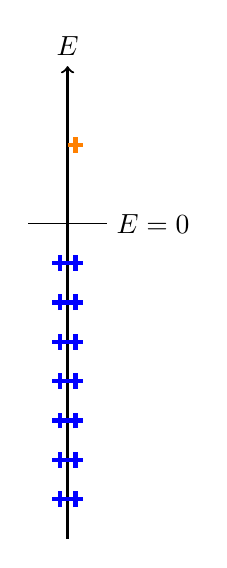
\begin{tikzpicture}

        % Disegna l'asse y
        \draw[->,thick] (0,-4) -- (0,2) node[above] {$E$};
        \draw(-.5,0) -- (.5,0) node[right]{$E=0$};
        
        % Disegna le x piccole e blu sulla parte negativa dell'asse y
        \foreach \y in {-0.5,-1,-1.5,-2,-2.5,-3,...,-3.5} {
          \draw[blue,ultra thick] (0,\y) -- ++(0.2,0);
          \draw[blue,ultra thick] (0,\y) -- ++(-0.2,0);
          \draw[blue,ultra thick] (0.1,\y-0.1) -- ++(0,0.2);
          \draw[blue,ultra thick] (-0.1,\y-0.1) -- ++(0,0.2);
        }
        \draw[orange,ultra thick] (0,1) -- ++(0.2,0);
        \draw[orange,ultra thick] (0.1,1-0.1) -- ++(0,0.2);
        
        \end{tikzpicture}
        \small A simple representation of the Dirac's sea idea. Blue crosses are the negative energy solutions while the orange ones are the positive.
}
To understand this interpretation we should introduce the concept of the \textbf{Dirac's sea}, or simply the collection of all the negative energy states, which, being experimentally inaccessible, are considered all full. All the regular particles that we observe are, energetically speaking, above this sea (since they have positive energy) and thus they cannot lose their energy and jump inside the sea (because it is already full).\\What could actually happen is to observe a \textbf{hole} in the sea, it is easy to see that this must be an antiparticle: in fact a particle (now with negative energy) could jump into the hole with the result that the energy and the charge of the system has to be those of the vacuum, thus zero.
\begin{equation*}
    \begin{cases}
        E(\text{hole})+(-E_p)=E_\text{Vac}=0\\
        Q(\text{hole})+Q=Q_{\text{Vac}}=0
    \end{cases}\quad\Rightarrow\quad\begin{cases}
        E(\text{hole})=E_p\\
        Q(\text{hole})=-Q
    \end{cases}.
\end{equation*} 
In this way we can see that holes has a positive energy (so that we don't contradict the fact that we don't measure negative energy particles) and the opposite charge of the regular particle, which corresponds to our experimental observation about antiparticles.\\
We could think of an antiparticle-particle couple as a negative energy state getting excited and thus jumping outside the sea creating a positive energy particle and a hole.\\
Notice that the sea should have an infinite energy, but we have set that to be zero, predicting the renormalization of the vacuum energy of quantum field theory. However, we will see that this interpretation will be replaced by the results of quantum field theory itself.\\

Let's study what happens to particles and antiparticles in the Dirac's equation. Introducing electromagnetic interactions we expect the Dirac's equation to hold both for positive charges $\psi$ and negative charges $\psi_C$:
\begin{equation*}
    [\gamma^\mu(\partial_\mu-ieA_\mu)+m]\psi=0,\qquad  [\gamma^\mu(\partial_\mu+ieA_\mu)+m]\psi_C=0.
\end{equation*}
To obtain these couple of equations we can try to take the complex conjugate of the one for positive cherges:
\begin{equation*}
    [\gamma^{\mu*}(\partial_\mu+ieA_\mu)+m]\psi^*=0,
\end{equation*}
this equation suggests that we have to find a proper way to transform $\gamma^{\mu*}$ to the normal ones. Introducing a transformation $\mathcal{A} $ such as:
\begin{equation*}
   \mathcal{A} \gamma^{\mu*}\mathcal{A} ^{-1}=\gamma^\mu\quad\Rightarrow\quad[\mathcal{A} ^{-1}\gamma^{\mu}\mathcal{A} (\partial_\mu+ieA_\mu)+m]\psi^*=0,
\end{equation*}
by multiplying all the equation, to the left, by $\mathcal{A} $ we get the equation for the antiparticle, which is thus described by $\psi_C=\mathcal{A} \psi^*$.\\
However, is usually done is to find $\psi_C$ using $\bar\psi$:
\begin{equation*}
    \psi_C=\mathcal{A} \psi^*=\mathcal{A}\beta\beta \psi^*=\mathcal{A}\beta(\psi^\dagger\beta)^t=\mathcal{A}\beta\bar\psi^t, 
\end{equation*}
we thus define the charge conjugation operation $\mathcal{C} =\mathcal{A} \beta$.\\
The transformation law for $\gamma^\mu$ now reads:
\begin{equation*}
    \gamma^mu=\mathcal{C} \beta\gamma^{\mu*}(\mathcal{C} \beta)^{-1}=\mathcal{C} \beta\gamma^{\mu*}\beta\mathcal{C} ^{-1}=-\mathcal{C} \gamma^{\mu t}\mathcal{C} ^{-1},
\end{equation*}
since $\beta\gamma^{\mu}\beta=\gamma^{\mu\dagger}$.\\
This suggests that $\gamma^0$ and $\gamma^2$ should anticommute with $\mathcal{C}$, while the other two should commute
\begin{equation*}
    \mathcal{C} \gamma^\mu\mathcal{C} ^{-1}=-\gamma^{\mu t}=\begin{pmatrix}
        -\gamma^0\\\gamma^1\\-\gamma^2\\\gamma^3
    \end{pmatrix}\qquad\Rightarrow\qquad\mathcal{C} =\gamma^0\gamma^2.
\end{equation*}
Here we have used that $\gamma^0$ and $\gamma^2$ are symmetric while the other two are antisymmetric.\\

Let's study what happens to a Weyl's spinor under this transformation:
\begin{equation*}
    (\psi_L)_C=\mathcal{C} \bar\psi_L^t=\mathcal{C} (\beta P_L\psi^*)=\mathcal{C} P_R(\beta \psi^*)=P_R(\psi_L)_C,
\end{equation*}
so the charge conjugate of a left-handed spinor is right-handed (and vice versa).
\section{Propagator of the Dirac's equation}
We want to find the propagator of the Dirac's equation: such fucntion, as we already discussed for the Klein-Gordon equation, is a green function of the differential equation that we are studing. Such function should then satisfy:
\begin{equation*}
    (\not\partial+m)S(x-y)=\delta^4(x-y).
\end{equation*} 
Again, to solve this differential equation we can use the Fourier transform:
\begin{equation*}
    S(x-y)=\int\frac{d^4p}{(2\pi)^4}e^{ip(x-y)}\tilde{S}(x-y),
\end{equation*}
plugging it into the above differential equation we get
\begin{equation*}
    (i\not{p}+m)\tilde{S}(p)=\mathds{1}.
\end{equation*}
This algebraic equation leads to the solution:
\begin{equation*}
    \tilde{S}(p)=\frac{-\not{p}+m}{p^2+m^2},
\end{equation*}
which should be used with the Feynman prescription in order to get the propagator:
\begin{equation*}
    -iS(x-y)=\int\frac{d^4p}{(2\pi)^4}e^{ip(x-y)}\frac{-\not{p}+m}{p^2+m^2-i\epsilon}.
\end{equation*}  
\section{Action of the Dirac's equation}
We will end our discussion on the Dirac's equation by studying the action that, through the principle of least action, leads to such equation. Being a complex field, the action functional had to depend on both the $\psi$ and its conjugate, however, in order to obtain a fermionic scalar Lorentz invariant, it will depend on $\bar\psi$:
\begin{equation}
    \mathcal{S} [\psi,\bar\psi]=\int d^4x[-\bar\psi(\not{\partial}+m)\psi].\label{DiracEqAction}
\end{equation}
Evaluating the variation $\delta\mathcal{S} $, under the assumption that the fields vanish on the frontier of the domain, we can check that this is actually the right action:
\begin{align*}
    \delta\mathcal{S} &=\int d^4x[-\bar\delta\psi(\not{\partial}+m)\psi-\bar\psi(\not{\partial}+m)\delta\psi]\\
    &\text{Integrating by parts}\\
    &=\int d^4x[-\bar\delta\psi(\not{\partial}+m)\psi+(\bar\psi\not{\partial}+m\bar\psi)\delta\psi-\partial_\mu(\bar\psi\gamma^\mu\delta\psi)]=0,
\end{align*}
here the last term vanishes due to boundary conditions while the other two must vanish giving the equations of motion \eqref{DiracEquation}.\\

We can now use the Nother's theorem on this action. The action \eqref{DiracEqAction} is clearly (being a bilinear) invariant under transformations of the $U(1)$ group $\psi\rightarrow\psi'=e^{i\alpha}\psi$.\\
The variation of the field under this transformation is
\begin{equation*}
    \delta_\alpha\psi=\psi'-\psi=(1+i\alpha+O(\alpha^2))\psi-\psi\backsimeq  i\alpha\psi,\qquad \delta_\alpha\bar\psi\backsimeq  -i\alpha\bar\psi,
\end{equation*}
by promoting $\alpha$ to a function of the coordinates, the variation of the action reads:
\begin{equation*}
    \delta_{\alpha(x)}\mathcal{S}=\int d^4x(-\partial_\mu)(\bar\psi\gamma^\mu\psi\alpha(x))=-\int d^4x[(\partial_\mu\alpha)(i\bar\psi\gamma^\mu\psi)+\alpha\partial_\mu(i\bar\psi\gamma^\mu\psi)]=0,
\end{equation*}
which gives us the conserved current $\partial_\mu J^\mu=\partial_\mu(i\bar\psi\gamma^\mu\psi)=0$.
This current can be generalized to the symmetry $U(1)\times SU(N)$ of a system of $N$ particles.\\

Let's now study the action that can describe the chiral nature of fermions. \\
In order to do so we should study how different Weyl components mix in bilinear products (remind that $P^2_{R/L=P_{R/L}}$):
\begin{align*}
    \bar\psi\psi_{R/L}&=\bar\psi\frac{1\pm\gamma^5}{2}\psi=\psi^\dagger\beta\bigg(\frac{1\pm\gamma^5}{2}\bigg)^2\psi=\psi^\dagger\frac{1\mp\gamma^5}{2}\beta\frac{1\pm\gamma^5}{2}\psi\\&=\bar\psi_{L/R}\psi_{R/L},\\
    \bar\psi\gamma^\mu\psi_{R/L}&=\bar\psi\gamma^\mu\frac{1\pm\gamma^5}{2}\psi=\psi^\dagger\beta\gamma^\mu\bigg(\frac{1\pm\gamma^5}{2}\bigg)^2\psi=\psi^\dagger\frac{1\pm\gamma^5}{2}\beta\gamma^\mu\frac{1\pm\gamma^5}{2}\psi\\&=\bar\psi_{R/L}\gamma^\mu\psi_{R/L}.
\end{align*}
Using these observations it is straight forward to see that the action \eqref{DiracEqAction} reads:
\begin{equation}
    \label{DiracEqActionWeyl} \mathcal{S}=\int d^4x[-\bar\psi_{L}\gamma^\mu\partial_\mu\psi_{L}-\bar\psi_{R}\gamma^\mu\partial_\mu\psi_{R}-m(\bar\psi_{L}\psi_{R}+\bar\psi_{R}\psi_{L})].
\end{equation}
Notice that components gets mixed only by the mass term of this equation, for this reason we cannot describe massive particles that are fully right or left-handed.\\

Lastly we should study a particular mass term that we could add to this action, called \textbf{Majorana mass}:
\begin{equation}\label{MajoranaMassLagr}
    \mathcal{L}_{\text{Maj}}=\frac{M}{2}\psi^t\mathcal{C} ^{-1}\psi+\frac{M}{2}(\psi^t \mathcal{C} ^{-1}\psi)^\dagger,
\end{equation}
this term is Lorentz invariant, since an infinitesimal Lorentz transformation is given by (remind that $\mathcal{C} ^{-1}\gamma^\mu\mathcal{C} =-\gamma^{\mu\ t}$)
\begin{align*}
    \delta\psi&=\frac{i}{2}\omega_{\mu\nu}\Sigma^{\mu\nu}\psi,\\
    \delta\psi^t&=\frac{i}{2}\omega_{\mu\nu}\psi^t\Sigma^{\mu\nu\ t}=-\frac{i}{2}\omega_{\mu\nu}\psi^t\mathcal{C}^{-1}\Sigma^{\mu\nu}\mathcal{C},
\end{align*}
each variation cancels out the other. This term breaks the $U(1)$ symmetry of the system, since a constant phase would appear in the action. This can be used to reproduce particles that, experimentally, break this symmetry. We could thus define a \textbf{Majorana spinor}
\begin{equation*}
    \mu(x)=\psi_L(x)+(\psi_L)_C(x),
\end{equation*}
which can describe particle with a physical mass given by $\mu^2_{1,2}=m^2+M^2$.







